\documentclass[journal,12pt,onecolumn]{IEEEtran}
\usepackage{cite}
\usepackage{caption}
\usepackage{graphicx}
\usepackage{amsmath,amssymb,amsfonts,amsthm}
\usepackage{algorithmic}
\usepackage{graphicx}
\usepackage{textcomp}
\usepackage{xcolor}
\usepackage{tfrupee}
\usepackage{txfonts}
\usepackage{listings}
\usepackage{enumitem}
\usepackage{mathtools}
\usepackage{gensymb}
\usepackage{comment}
\usepackage[breaklinks=true]{hyperref}
\usepackage{tkz-euclide} 
\usepackage{listings}
\usepackage{gvv}
%\def\inputGnumericTable{}
\usepackage[latin1]{inputenc} 
\usetikzlibrary{arrows.meta, positioning}
\usepackage{xparse}
\usepackage{color}                                            
\usepackage{array}                                            
\usepackage{longtable}                                       
\usepackage{calc}                                             
\usepackage{multirow}
\usepackage{multicol}
\usepackage{hhline}                                           
\usepackage{ifthen}                                           
\usepackage{lscape}
\usepackage{tabularx}
\usepackage{array}
\usepackage{float}
\usepackage{marvosym}
\usepackage{float}
%\newcommand{\define}{\stackrel{\triangle}{=}}
\theoremstyle{remark}
\usepackage{circuitikz}
\captionsetup{justification=centering}
\usepackage{tikz}

\title{Matrices in Geometry 5.13.63}
\author{EE25BTECH11037 - Divyansh}
\begin{document}
\vspace{3cm}
\maketitle
{\let\newpage\relax\maketitle}
\textbf{Question: }
Let $\vec{M}=\myvec{\sin^4\brak{\theta} & -1-\sin^2\brak{\theta} \\ 1+\cos^2\brak{\theta} & \cos ^4\brak{\theta}} = \alpha \vec{I} + \beta\vec{M}^{-1} $\\
Where $\alpha = \alpha\brak{\theta}$ and $\beta = \beta \brak{\theta}$ are real numbers, and $\vec{I}$ is the $2 \times 2$ identity matrix.
If $\alpha^*$ is the minimum of the set $\brak{\alpha\brak{\theta}: \theta \in [0, 2\pi)} $ and $\beta^*$ is the minimum of the set
$\brak{\beta\brak{\theta} : \theta \in [0, 2\pi)}$. Then the value of $\alpha^* + \beta^*$ is
\begin{multicols}{4}
    \begin{enumerate}
        \item $-\frac{31}{16}$
        \item $-\frac{17}{16}$
        \item $-\frac{37}{16}$
        \item $-\frac{29}{16}$
    \end{enumerate}
\end{multicols}
\vspace{2mm}


\textbf{Solution:}
Using the Cayley-Hamilton Theorem, 
\begin{align}
    \vec{M}^2 - tr\brak{\vec{M}}\vec{M} + det\brak{\vec{M}}\vec{I}=0\\
    \implies \vec{M} -tr\brak{\vec{M}}\vec{I} + det\brak{\vec{M}}\vec{M}^{-1} =0
\end{align}
The given expression is
\begin{align}
    \vec{M} -\alpha\vec{I} - \beta\vec{M}^{-1} =0
\end{align}
On comparing, we get
\begin{align}
    \alpha = tr\brak{\vec{M}} \ , \ \beta = - det\brak{\vec{M}}\\
    \alpha\brak{\theta}=\sin^4\brak{\theta}+\cos^4\brak{\theta} = 1-2\sin^2\brak{\theta}\cos^2\brak{\theta}\\
    \implies \alpha = 1 -\sin^2\brak{2\theta}/2 \\
    \alpha^*  = min\brak{\alpha\brak{\theta}}= 1- 1/2 = \frac{1}{2} ,\\ \brak{\because \text{for minimizing $\alpha$,  $\sin^2\brak{2\theta}$ should be maximum}}\nonumber\\
    \beta\brak{\theta} = - det\brak{\vec{M}} = - \brak{\sin^4\brak{\theta}\cos^4\brak{\theta} + \sin^2\brak{\theta}\cos^2\brak{\theta} +2}\\
    \implies \beta = - \brak{ \brak{\sin\brak{2\theta}/2}^4 + \brak{\sin\brak{2\theta}/2}^2 + 2} \\
    \beta^* = - \brak{ \brak{1/2}^4 + \brak{1/2}^2 + 2}=--\frac{37}{16}\\
    \brak{\because \text{for minimizing $\beta$,  $\sin^2\brak{2\theta}$ should be maximum}}\nonumber
\end{align}
Now, 
\begin{align}
    \alpha^*+\beta^* = \frac{1}{2} - \frac{37}{16} = -\frac{29}{16}
\end{align}
Thus,  the correct option is option $4)$.\\
We get $\alpha^*, \beta^*$ at $\theta = \frac{\pi}{4}$, substituting this in $\vec{M}$, we get
\begin{align}
    \vec{M}=\myvec{\brak{\frac{1}{\sqrt{2}}}^ 4 & -1-\brak{\frac{1}{\sqrt{2}}}^2 \\  1+\brak{\frac{1}{\sqrt{2}}}^2 & \brak{\frac{1}{\sqrt{2}}}^ 4} = \myvec{\frac{1}{4} & \frac{-3}{2} \\ \frac{3}{2} &\frac{1}{4}}
\end{align}
Let us draw graphs to find $\alpha^*, \beta^*$:
\begin{figure}
    \centering
    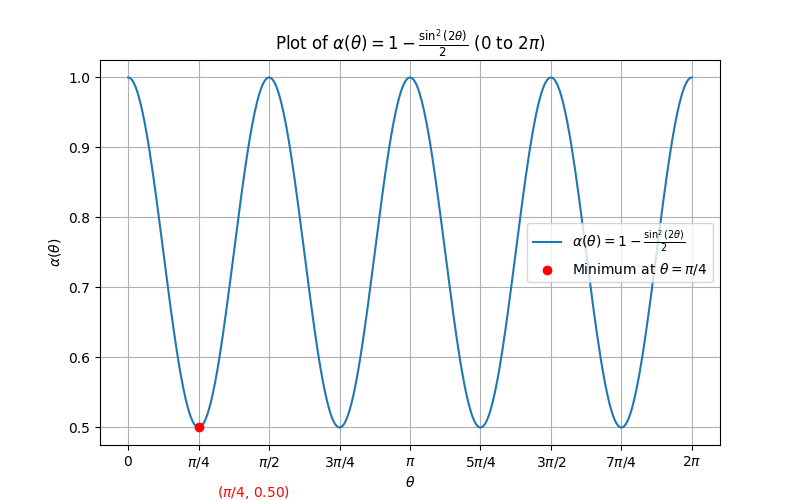
\includegraphics[width=0.5\columnwidth]{figs/alpha.png}
    \caption{Graph for $\alpha\brak{\theta}$}
    \label{fig:placeholder}
\end{figure}
\begin{figure}
    \centering
    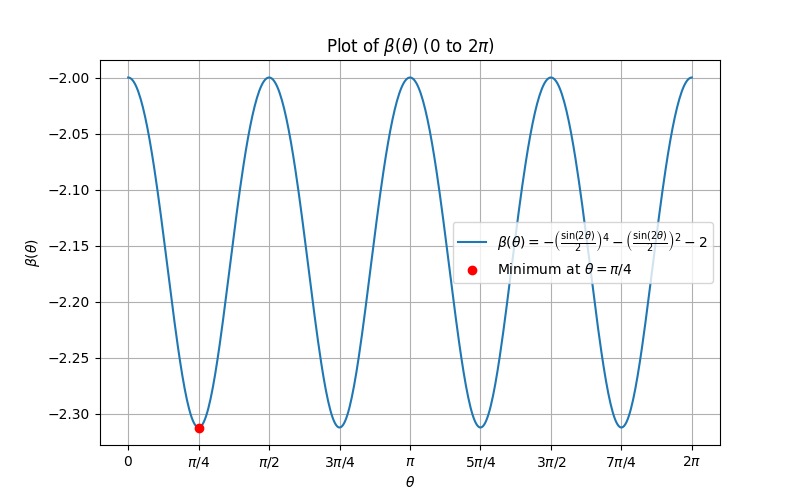
\includegraphics[width=0.5\columnwidth]{figs/beta.png}
    \caption{Graph for $\beta\brak{\theta}$}
    \label{fig:placeholder}
\end{figure}
\end{document}

